\documentclass{article}
\usepackage[a4paper, landscape, margin=1in]{geometry} % Landscape - horizontal layout
\usepackage{graphicx} % For including images
\usepackage{hyperref} % For hyperlinks
\usepackage{pgfplots} % For plots

% Configure
\pgfplotsset{compat=1.18}

% Title Information
\title{About Me}
\author{Lorena Dumba}
\date{\today}

% Data
\begin{filecontents*}{corn_data.dat}
Year Actual Estimate
1980 85  95
1985 98  115
1990 123 121
1995 110 123
2000 125 135
2005 170 155
2010 165 165
2015 184 185
2020 183 190
\end{filecontents*}

\begin{document}

% Title Slide
\begin{center}
    \huge{\textbf{About Me}}\\
    \vspace{1cm}
    \Large{Lorena Dumba}\\
    \vspace{0.5cm}
    \large{\today}
\end{center}
\newpage

% Introduction Slide
\section*{Introduction}
\begin{itemize}
    \item \textbf{Birthday:} February 7th
    \item \textbf{Hometown:} Belo Horizonte, Minas Gerais - Brazil
    \item \textbf{Program:} Plant Breeding and Genetics, Statistics
    \item \textbf{Expected Graduation:} August, 2027
\end{itemize}
\newpage

% Favorite Animal Slide
\section*{Favorite Animal}
\begin{center}
    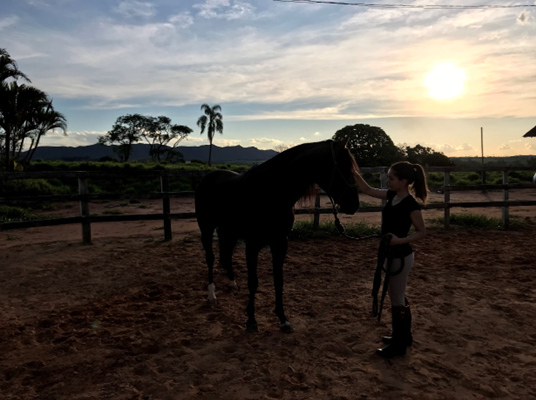
\includegraphics[width=0.6\textwidth]{horse.png}\\
    \vspace{0.5cm}
    \textbf{I love horses!}
\end{center}
\newpage

% Favorite Plot Slide
\section*{Favorite Plot}

\begin{center}
    \textbf{Corn Production in Nebraska: Actual vs. August Estimate}
\end{center}

\begin{figure}[h!]
    \centering
    \begin{tikzpicture}
        \begin{axis}[
            title={Corn Production: Actual vs. August Estimate},
            xlabel={Year},
            ylabel={Bushels/Acre},
            grid=major,
            legend pos=south east
        ]
            \addplot[blue, mark=*] table [x=Year, y=Actual, col sep=space] {corn_data.dat};
            \addplot[orange, mark=square*] table [x=Year, y=Estimate, col sep=space] {corn_data.dat};
            \legend{Actual, August Estimate}
        \end{axis}
    \end{tikzpicture}
\end{figure}

\begin{center}
    \textbf{Reference:} \url{https://www.nefb.org/08/23/2023/larger-crop-production-in-2023/}
\end{center}
\newpage

% CV Link Slide
\section*{CV Link}
\begin{center}
    \href{CV.pdf}{My CV}
\end{center}

\end{document}
